A poorly insulated, leaky cabin with interior temperature $T_i$ is impacted by both the cabin's heater, which supplies heat flow $\dot{Q}$, and outdoor ambient temperature $T_a$ as shown in the block digram below, where $\dot{Q}(s)$ is determined by a proportional controller and $R(s)$ represents the thermostat set point.

\begin{center}
	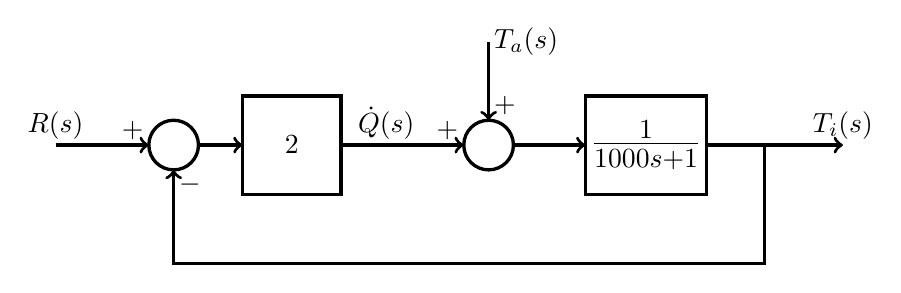
\begin{tikzpicture}[scale=1,inner sep=0pt,outer sep=0pt,very thick,
	sysblock/.style={draw,rectangle,inner sep=2pt,minimum width=1.25cm,minimum height=1.25cm,very thick}]
	\draw (2,0) node[draw,circle] (sum1) {$\rule{0pt}{18pt}$};
	\draw (3.5,0) node[sysblock] (Kp) {$2$};
	\draw (6,0) node[draw,circle] (sum2) {$\rule{0pt}{18pt}$};
	\draw (8,0) node[sysblock] (G) {\Large $\frac{1}{1000s+1}$};
	\draw[->] (.5,0) node[above=2pt] {$R(s)$} -- (sum1.180) node[above left=2pt] {$+$};
	\draw[<-] (sum2.90) node[above right=2pt] {$+$} -- ++(0,1) node[right=2pt] {$T_a(s)$};
	\draw[->] (sum1.0) --  (Kp);
	\draw[->] (4.7,0) node[above=2pt] {$\dot{Q}(s)$} (Kp) -- (sum2.180) node[above left=2pt] {$+$};
	\draw[->] (sum2) -- (G);
	\draw[->] (G) -- ++(2.5,0) node[above=2pt] {$T_i(s)$};
	\draw[->] (G) ++(1.5,0) -- ++(0,-1.5) -| (sum1.-90) node[below right=2pt] {$-$};
	\end{tikzpicture}
\end{center}

\begin{enumerate}[(a)]
	\setlength{\itemsep}{1pt}
	\setlength{\parskip}{0pt}
	\setlength{\parsep}{0pt}
	\item Find the transfer function from the ambient outdoor temperature $T_a$ to the indoor temperature $T_i$. 
	\item If a cold front suddenly moves in and the outdoor temperature changes by $-10^{\circ}$, that is, $T_a(t)~=~-10u(t)$, by how much will the indoor temperature $T_i(t)$ change in steady-state?
	\item Check your answer in Matlab using the transfer function \texttt{'sys'} you derived in (a) and \texttt{'step(-10*sys)'}.
\end{enumerate}
